\documentclass{book}
\usepackage{graphicx}
\begin{document}
\setcounter{chapter}{2}
\chapter{system and software life cycle processes}
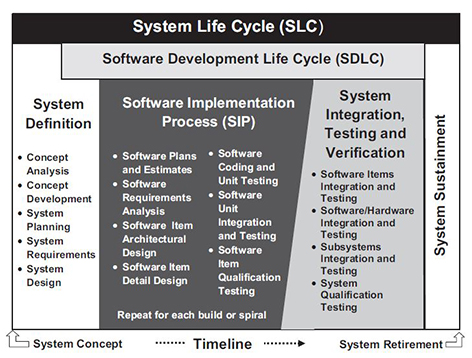
\includegraphics{1.jpg}

\textbf{Figure 3.3 Overview of the System Life Cycle.}

%paragraph1
The focus of the Project Charter is on all aspects of the overall system solution being considered including:

-Required functionality, operational concepts and capabilities

-Technology development strategies

- Alternative architectures and candidate solutions

- Risk reduction activities and control schemes

- Initial software development planning

- Initial estimated system costs and benefits

%paragraph2
\textbf{Software Subject Matter Experts.} During System Definition, the entire focus is at the system level. Essentially all modern day systems have a major Software Component, so Software Subject Matter Experts (SSMEs) are needed as technical support for all software-related issues. Their challenges are:

- Early recognition of system capabilities that will or may require software contributions during system development, and

- Assessment of the feasibility of the proposed software solutions. System and Software Designers evaluate actual alternatives in later milestones. However, infeasible or unviable capabilities or implementation options should be identified and modified or eliminated as early as possible.

In addition, SSMEs are needed for estimating software development costs. The initial cost estimates include an analysis of the amount of software for new code to be developed as well as the potential for reused code. Once the software size is estimated for each type of software, an independent analysis translates software size estimates into more accurate cost estimates using software cost estimation models. The cost estimates are used to help decide if the proposed project should proceed.

%paragraph3

\textbf{System Capabilities Documents} For large systems, initial capabilities documents, often called Concept of Operations(CONOPS), are often prepared. Although they may have limited software content, Software Engineers must identify software implications of the required user capabilities. The initial and preliminary System Definition tasks should not be confused with the detailed system requirements and System Design tasks covered in Chapter 10. Section 12.5 discusses software involvement during system concept analysis.

%paragraph4\
\setcounter{section}{3}
\section{Software Development Life Cycle Process}

 The Software Development Life Cycle, as shown in Figure 3.3, starts during System Definition and ends at the start of System Sustainment. Embedded within the SDLC are: part of the System Definition task; the entire SIP; and the System Integration, Testing and Verification process Figure 3.4 is an expansion of Figure 3.3 as it is a more detailed graphical representation of the relationship between the SLC, SDLC, SIP and the System Integration and testing buildup prior to transition to operations and sustainment.
There is a lot going on in Figure 3.4; take time to understand it as that would be a giant step forward in understanding the overall processes.

Figure 3.4 shows the SIP embedded within the Software Development Life Cycle. The SIP for each build consists of seven sequential activities (with appropriate iterations). The example in Figure 3.4 involves two Software Items (SIs) under development including three builds in SI-1. The SIP covers the full cycle of software implementation tasks performed for each build (or spiral) from initial software build planning to Software Item Qualification Testing (SIQT).

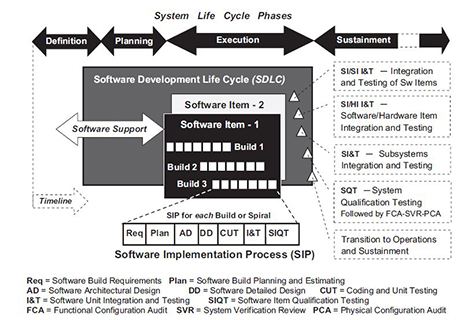
\includegraphics{2.jpg}

\textbf{Figure 3.4 Overview of the System and Software Development Life Cycles.}

%paragraph5
\section{Software Implementation Process}

Figure 3.5 depicts the full software integration and testing process. The SLC phases shown at the top of Figure 3.5 are a toplevel system acquisition perspective. The seven SIP activities are part of the Software Engineering Domain, and those activities are described in depth in Chapter 11. The SIP is repeated for each build or spiral and may be repeated multiple times during System Sustainment to implement new functions and make needed modifications. The seven SIP activities are:

- Software Build Requirements: Software Systems Engineering should define the level of requirements satisfaction needed by each build or increment to implement a specified level of system functionality.Within a subsystem, additional influences may dictate when capabilities are needed. This may include such factors as developing required software infrastructure or addressing areas of high-complexity. Also, naming conventions for each build must be established up front by assigning unique alphanumeric designations.

-Software Build Planning and Estimating: Software build planning is covered in Subsection 5.1.4 and software estimating has its own chapter (14). Software project planning and estimating are considered (in this Guidebook) as part of the Project Management Domain. Regardless of where these activities appear in the Guidebook, software planning and estimating are essential components of the development process. The re-planning activity is a critical ongoing task because changes almost always need to be made during development.

- Software Architectural Design: Architectural (or preliminary) Design precedes Detailed Design. The objective of SI Architectural Design is to describe the high-level organization of the SIs in terms of the planned functionality and relationships of the Software Units (SU).

- Software Detailed Design: The objective of SI Detailed Design is to determine and define the implementation details for each SU. It involves decomposing the SIs from the SI Architectural Design into the lowest level SUs in sufficient detail to map the design to the features of the selected programming language, the target hardware, operating system, and network architecture.


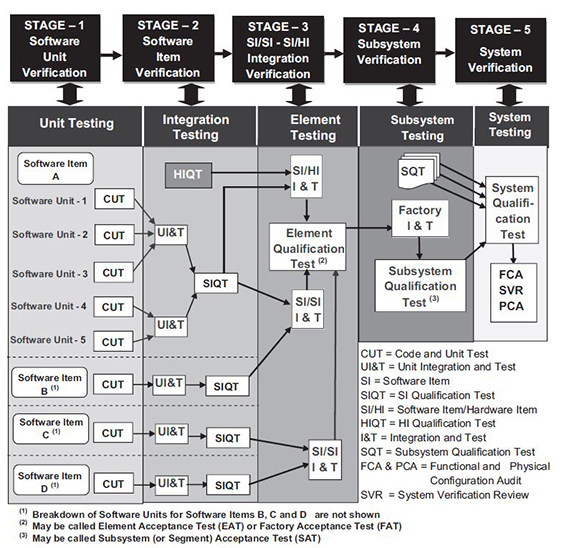
\includegraphics{3.jpg}

\textbf{Figure 3.5 Software integration and testing process.}

- Coding and Unit Testing: Converts the SU Detailed Design into computer code and databases that are inspected, unit tested, and confirmed as responsive to the design.

-Software Unit Integration and Testing: A systematic and iterative series of integration builds of SUs that have successfully completed Code and Unit Test, and building them up to a higher level SU, or SI, for the current build (see Sections 3.6 and 11.5).

- Software Item Qualification Testing: Demonstrates that the Software Item meets the system and interface requirements allocated to the SI being tested. (see Sections 3.6 and 11.6).

%paragraph6
\section{System Integration, Test and Verification Process}

The System Integration, Testing and Verification process is embedded within the SDLC as shown in Figures 3.3 and 3.4. The system IT and V process involves activities where individual software modules are combined and then tested and verified as a group. It occurs after unit testing of the code but before System Qualification Testing. Integration testing takes, as its input, software modules that have been unit tested, it groups them in larger aggregates, applies tests defined in the Software Test Plan (STP) to those aggregates, and delivers as its output the integrated system ready for system testing. There may be a separate Integration Test Plan, or it may be incorporated in the STP.

Discussion of the system IT and V, presented in Section 3.6 below, includes the IT and V stages as well as the IT and V process. IT and V is also described as part of the Systems and Software Engineering Domains in Chapters 10 and 11 including:

- Software Unit Integration and Testing (Section 11.5)

- Software and Hardware Item Integration and Testing(sections 10.3 and 11.7)

- System Qualification Testing (Section 10.4)

The system IT and V approach must be consistent and compliant with the system-level integration and verification test plan often called the system Master Test Plan (MTP). The rationale for software testing is based on an incremental buildup of tested requirements with a simultaneous incremental verification buildup. An example of the software integration and testing process is graphically depicted in Figure 3.5 showing a systematic and incremental buildup of testing software requirements. The generic software IT and V process normally involves five testing stages as shown in Figure 3.5.

%paragraph7
\section{System Sustainment}
The last activity of the System Life Cycle is System
Sustainment. This activity is not covered in Chapter 3
because Chapter 16 is devoted to the sustainment activities
(often called maintenance), and that chapter is focused on
the management issues encountered during sustainment.
Software Sustainment includes the processes, procedures,
people, materiel and information required to fully support,
maintain and operate the software portions of a system over
a long period of time (sometimes decades). Most Software
Engineering literature is focused only on software development
activities, but sustainment is actually the longest and
most expensive activity of the System Life Cycle. From the user’s
standpoint, it may also be considered the most important
activity.
%paragraph8

\section{System Critical and Support Software Processes}
As discussed in Section 1.8, every software entity must be
assigned a class and category because:

Not every software entity needs to have the full set
of documentation, the full set of reviews, the full set
of metrics, and the same level of testing.

Significant savings can be realized if software entities can
be placed into a class that does not require the same level of
attention required by software that is critical to full functionality
and performance of the system. Section 1.8 described
three generic classes of software in a software-intensive system:

- System Critical Software (SCS) discussed in Subsection
3.8.1

- Support Software (SS) discussed in Subsection 3.8.2

- Commercial Off-the-Shelf or Reuse Software (C/R) discussed
in Section 9.7

\subsection{Development Process for System Critical Software}
SCS was defined in Subsection 1.8.1 as consisting of all
applications software used to perform real-time operations
and non-real-time functions implicitly required to implement
system functionality allocated to software. Figure 3.6 is an
example graphical overview of a software development process
for the SCS class of software. Tailor it for your project.

The SCS process is a comprehensive process since it provides
the critical application software functionality. SCS
development must support the development of as many SIs
and builds as needed to meet customer requirements, contract
milestones and system objectives. As shown in Figure 3.6, the
SCS development process begins with requirements analysis
and definition for each SI using system-level documents, such
as the Technical Requirements Document (TRD) and the subsystem-
to-subsystem Interface Specifications.

Requirements from these specifications are allocated to
software and hardware, and the allocated software requirements
are functionally decomposed, elaborated and documented
in the Software Requirements Specification (SRS)
and the Interface Requirements Specification (IRS). For the
SCS class, Detailed Design, coding, integration, and testing
activities are performed for each SI within each build.
Once the SIs are integrated and tested for a build, the build
is delivered, along with the Software Version Description
(SVD), to the cognizant Software Development Library
for Configuration Management control as discussed in
Section 6.3.

\subsection{Development Process for Support Software (SS)}

Support Software (SS) was defined in Subsection 1.8.2 as software
that aids in the development of hardware and software,
integration, qualification, operations, test and maintenance.
Figure 3.7 is an example graphical overview of a software
development process for the SS class of software.

Although Support Software operates only in non-operational
environments, the SS-1 category normally requires
the same level of documentation as SCS software. However,
reviews for the SS-1 category may not be as formal or as frequent
as it is for SCS. The principal differences between the
examples for SCS software (Figure 3.6), and SS software
(Figure 3.7) processes, is that for (SS-1):

- There is no formal Software Specification Review
(SSR), PDR, CDR, IRR, PTR and BTR as shown
for System Critical Software; they are replaced by
Technical Interchange Meetings (TIMs).

- The Architecture and Detailed Design phases are
merged and followed by a TIM.

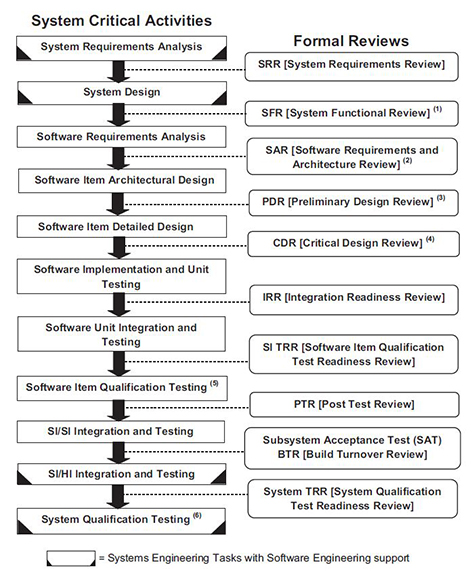
\includegraphics{4.jpg}

\textbf{Figure 3.6 System Critical Software development process. (1) The SFR was formerly called the System Design Review
	(SDR). (2) SAR and PDR may be combined for Object-Oriented development because requirements definition and
	Architectural Design are usually iterative. The SAR was formerly called the Software Specification Review. (3) An
	optional SBRAR [Software Build Requirements and Architecture Review] may be held in addition to the PDR. (4) An
	optional SBDR [Software Build Design Review] may also be held in addition to the CDR. (5) Software Item Qualification
	Testing may be performed within each build. (6) SQT can be followed by FCA, SVR and PCA prior to transition to
	operations.}

The SS-2 development process should be expected to
be similar to the SS-1 process, but much less stringent. The
principal differences between SS-1 and SS-2 software are:

- SS-2 requirements information is normally maintained
in a Requirements Database and referenced in SDFs,
just as it is for SS-1, but formal preparation of the SRS,
SDD and IDD is usually not required for the SS-2 class.

- Informal SI and software build test descriptions
and test results are maintained in SDFs. However,
formal STP, STD and STR documents are usually not
required for the SS-2 class.

- TIMs performed for SS-1 may be replaced by Peer
Reviews for the inspections and verifications of work
products developed for the SS-2 class.

- Applicable software metrics data should be collected
for SS-2 software, but the metrics data set and the
reporting frequencies should be significantly reduced
for the SS-2 class.









\end{document}